\subsection{Analysis} % (fold)
\label{sub:analysis}

% TODO: spatio-temporal queries

analysis: determine, change, evaluate

analysis methods
  spatial analysis
  temporal analysis
    time series analysis
    process analysis      (modification modeling + future forecasting)
  attribute analysis
alteration of \cite[p. 128]{ott2001time}

spatial queries
  query of spatial properties and attribute values
  e.g. size of Germany in 1871
thematic queries
  query objects based on certain criteria (spatial and attribute)
  multi-criteria analysis
  e.g. all democratic countries larger than 10.000 km²
statistical analysis
  artithmetic calculation and classification of characteristics of objects
  univariate, multivariate investigation
  e.g. What was the population density in Germany in 1945 compared to 1995
overlay/split
  aggregation and splitting of spatial components based on the layer principle
  e.g. Germany in 1945 gets split up into FRG and GDR by one polyline (inner German border) and one polygon (West Berlin)
geometric-topological operations
  analyze the neighborhood relations between geometric objects
  e.g. is the geometry all countries at time point 1991 strictly connected?
temporal analysis
  using spatial and temporal operators in figure
  %\ref{fig:spatial_temporal_operators}
  e.g. in which year did the largest amount of border changes happen?
\cite[p. 129-140]{ott2001time}

Multivariate Historical-Geographical Model
  multivariate
    features of a spatial object
    connection between temporal development of features
  geographical model
    location (geometry)
    neighborhood relation (topology)
  historical model
    object at different points in times
  \cite[p. 128]{ott2001time}
  % \cite Kilchenmann 1992

Spatial Queries / Operators
  and     intersection
  not     difference
  or      (cascaded) union
  xor     (inverted) symmetric difference

Temporal Queries / Operators

temporal logic
  rules and symbols
  represent time
  reason about time
  temporal operators
  ??? detail?
  % \cite Hodkinson and Reynolds 2006

  trajectories
    sequence of 2D or 3D locations of an object

Spatio-Temporal Queries / Operators
  when + where -> what
  when + what -> where
  where + what -> when
  % \cite Peuquet 1994


% ------------------------------------------------------------------------------
A GIS shall solve the problem for a user or answer his or her research question. Given a well-filled database with a working DBMS, the data might not answer the research question directly. It has to be sorted, selected or classified in order to convey the required information. For this process there are \emph{spatial operations} on the data in the system. Several operations can be applied in a certain order
\cite[pp. 321-325]{bolstad2008gis}.
Both spatial and attribute data are analyzed to combine the dimensions \emph{where?} and \emph{what?} in order to answer the ultimate question \emph{why?} something is the way it is
\cite[p.xii-xvi]{knowles2002past}.

An example is a system visualizing social developments on Earth. The researcher wants to divide the world into five regions with a similar life expectancy to see if there are spatial discrepancy of advances in global health. He or she has a GIS with all countries and their current life expectancy stored. In order to answer his or her research question, the following steps may be required

\begin{enumerate}
  \item Extract the life expectancy value per country.
  \item Classify the values on a discrete scale from very low to very high and put each country into one of the five classes.
  \item Unify neighboring countries that are in the same class to get five world regions.
  \item Name the five world regions.
  \item Apply a color scheme to the classification and set the background color for each of the five world regions.
  \item Create a legend with the classification and the explanation of the symbols.
  \item Present the resulting map on the screen.
\end{enumerate}

There are special operations for raster data, e.g. spatial interpolation, and for vector data.

Only explain those later that are really important!

graph / network analysis
  what is the shortest way from A to B?
  what is the fastest route from A via B1, B2, ..., Bn nack to A? (TSP)

Polygon geometry
  intersection, (cascaded) Union, (symmetric) difference

Polygon Clipping
  Sutherland-Hodgeman
  Weiler-Atherton

Topology analysis
  test for consistency, connectedness and completeness of topology

% subsection analysis (end)

% ------------------------------------------------------------------------------
\subsection{Presentation} % (fold)
\label{sub:presentation}

spatio-temporal visualization
-----------------------------

spatial domain
  2D: map, different projections
  3D: globe

temporal domain
  linear time
    time line
    time series: graph (t,y coordinate system)
    2.5D map: temporal dimension on z axis or on surface
    space-time path
  cyclic time
    time series: polar diagram
    time wheel
  both
    mono-temporal: one layer -> one time point
    multi-temporal: one layer -> multiple time points
\cite[p. 144]{ott2001time}

direct display of time on a map
  choropleth maps
  temporal diagrams
  change indicators

display mechanisms for visualizing temporal change
  change data         additional to base map (diagrams, texts)
  static symbols      thematic map, symbols: dates, routes, developments
  time sequence maps  mono-temporal maps in sequence
  animations          interactive visualization of time and space and attributes
\cite[p. 146-147]{ott2001time}


other approaches
  scatterplot               variation of two variables over time
  parallel coordinate plot  variation of multiple variables over time
  time series graph         variation of one variable over time

visualization in a way that people can understand it
  self-organizing map (SOM) nD variables -> 2D space + 2D color scheme
  % \cite Guo et al 2006


Scivis vs. Infovis

list of all possible spatial presentations -> only focus on maps
list of all possible temporal presentations -> only focus on timelines

Cartographic visualizations are the interface between the GIS and the human. A map is is the common form. It is a discrete graphical expression of the continuous real world. The creation of a map is not just a scientific, but also a creative process: The form, function and interaction methods shall follow the purpose of the usage of the map.

There is no fixed guideline how to properly design a map, but there are typical elements that are part of every cartographic visualization.The main element is the map itself, using a specific map projection
% (see section \ref{ssub:map_projections})
, a scale and an initial center point. A map is typically structured in a \emph{layer} principle. Each layer is a transparent film showing one specific aspect, e.g. a physical layer showing coastlines, mountains or forests, a political layer showing international borders or a cultural layer showing cities or population densities. The layers are interchangeable, can be switched on and off and serve to serve a different visualization purpose. The map is designed using a certain color scheme, fonts and signatures for all the objects on the map.

Additionally there can be a \emph{title} describing the purpose of the map. A \emph{legend} including the scale bar and north arrow shall explain all symbols used on the map and give orientation. Depending on the degree of interactivity, there can be \emph{menus} with different visualization options, e.g. panning and zooming on the map, switching map layers on and off or changing the color scheme of the map.
\cite[pp. 159-166]{bolstad2008gis}

% example of a good map

The main goal of map design is to give the user nothing but the necessary information he needs to satisfy his or her information need. The cartographer shall use techniques of \emph{cartographic generalization} to minimize information on the map and maximize the knowledge to be extracted from the map. Simplification, smoothing or aggregation help to reduce amount of information. Enlarging, widening or displacement help to focus on the important areas of the map. Selection and classification help the user to get an overview of the information.
\cite{krygier2005making}

Leaflet.js is ``an open-source JavaScript library for mobile-friendly interactive maps''
\footnote{
  \textit{Leaflet - JavaScript library for interactive maps},
  URL: \url{http://leafletjs.com/},
  last access: 02.11.2015
}
that offers functionality to embed a map with a chosen projection in an HTML document, use own map tiles, symbols and markers on the map and tools for zooming and panning.
The same service is provided by \emph{OpenLayers}, a ``A high-performance, feature-packed library for all your mapping needs''
\footnote{
  \textit{OpenLayers 3 - Welcome},
  URL: \url{http://openlayers.org/},
  last access: 02.11.2015
}, just with more features and users.


% ------------------------------------------------------------------------------
\subsubsection{Maps} % (fold)
\label{ssub:maps}


maps are means and products of GIS

scientific visualization vs. information visualization
  tangible objects            abstract concepts
  with inherent form          without inherent form
  e.g. CT scan of human body  e.g. flow of refugees
-> 3D globe: inherent form, direct representation of Earth -> scientific visualization
-> 2D map and time: no inherent form resp. abstract concept
=> information visualization

tasks of visualization
  present (what? where? when? how?)
  analyze (e.g. what is the best? where is the most? when was the first?)
  explore (why?)
% \cite Kraak 1999

interactive map enhances human cognition (panning, zooming, changing map layers, time point, data source, ...) and lets him gain knowledge about the domain

maps contain symbols and elements
  ... blaaa ...

traditional paper maps vs. modern digital maps
\begin{table}[ht]
\centering
\begin{tabular}{llp{1em}ll}
    \toprule
    \multicolumn{2}{c}{classical map} & & \multicolumn{2}{c}{modern digital map} \\
    character & restriction & & character & improvement \\
    \midrule
    static & only discrete point in time & & dynamic & higher sample rate for continuous processes \\
    isolating & only part of geographical space in 2D & & multi-dimensional & multiple levels of detail, possibility for representation of elevation and temporal dimension \\
    selective & only one layer & & inclusive & change layers and perspectives \\
    passive & only sending information & & interactive & direct manipulation and exploration \\
    \bottomrule
\end{tabular}
\caption{Innovation of modern digital maps}
\small{alternation of \cite{karcher} and \cite[p. 145]{ott2001time}}
\label{tab:maps_restrictions}
\end{table}

modern digital maps can show changes in time and space due to their dynamic, multi-dimensional, inclusive and interactive nature.


\paragraph{Map Projections} % (fold)
\label{par:map_projections}

One task of a HGIS is to visualize the Earth on a map. Since the Earth is an inhomogeneous three-dimensional shape but the output medium is a two-dimensional computer screen or piece of paper, it has to be transformed.

Based on the geodetic datum a three-dimensional representation of the Earth in form of a globe would be a possible medium to view the planet. When seen perpendicular onto the world, a globe represents sizes, shapes, distances and directions of objects close to the viewpoint with a reasonable accuracy. However, they are very space-consuming and cumbersome. For a precise measurement of distances, following a route or examining a terrain model, the globe would have to be very large. Therefore, the desired medium for practical purposes is a two-dimensional map.

The basic problem to be solved is that the Earth is a spherical object, its surface is curved and it is therefore not straightforward to project it onto a flat 2D map. The meridians which are lines of equal value converge at the poles. Neighboring meridians (distance: 1\degree) have a distance of 111 km at the Equator and 0 km at the poles. They do not form a right-angled grid with the parallels and therefore no Cartesian coordinate system. This is the reason why the geometries of the spherical Earth will be distorted when displayed on a flat 2D Cartesian coordinate system. \cite[p.79]{bolstad2008gis}

% \begin{figure}[ht]
%   \centering
%   \includegraphics[width=0.66\textwidth]{graphics/basics/distortion}
%   \caption{Distortion visualized by circles on a 2D map as a Cartesian coordinate system}
%   (on the 3D Earth all circles have the same size)
%   \label{fig:distortion}
% \end{figure}

There are two main classifications of map projections: The \emph{projection family} with respect to the geometric shape used for the transformation: \emph{cylindrical}, \emph{conical} and \emph{azimuthal} or \emph{planar projection}). Secondly, the \emph{distortion characteristics} with respect to the map property that is preserved. There are \emph{equivalent}, \emph{conformal}, \emph{equidistant}, \emph{zenithal} and compromise projections. Most families and characteristics can be mixed, e.g. it is possible to create a cylindrical, a conical and an azimuthal equivalent map projection
\cite{mapProjectionKrygier}.


\paragraph{Projection Families} % (fold)
\label{subp:projection_families}

The basis of geometrical map projections are \emph{developable surfaces} onto which the ellipsoidal model of the Earth is projected. The are mainly three geometric shapes that are used as reference surfaces: cylinders, cones and planes. The model is fitted in or on the surface touching it in at least one point or line. The idea is that there is a projection source from which rays are shot through the ellipsoid on the surface, projecting each point of the ellipsoid onto the surface (as seen in figure \ref{fig:projections}). This principle is known from the ray casting technique in computer graphics
\cite{mapProjectionGeokov}.

\begin{figure}[ht]
  \centering
  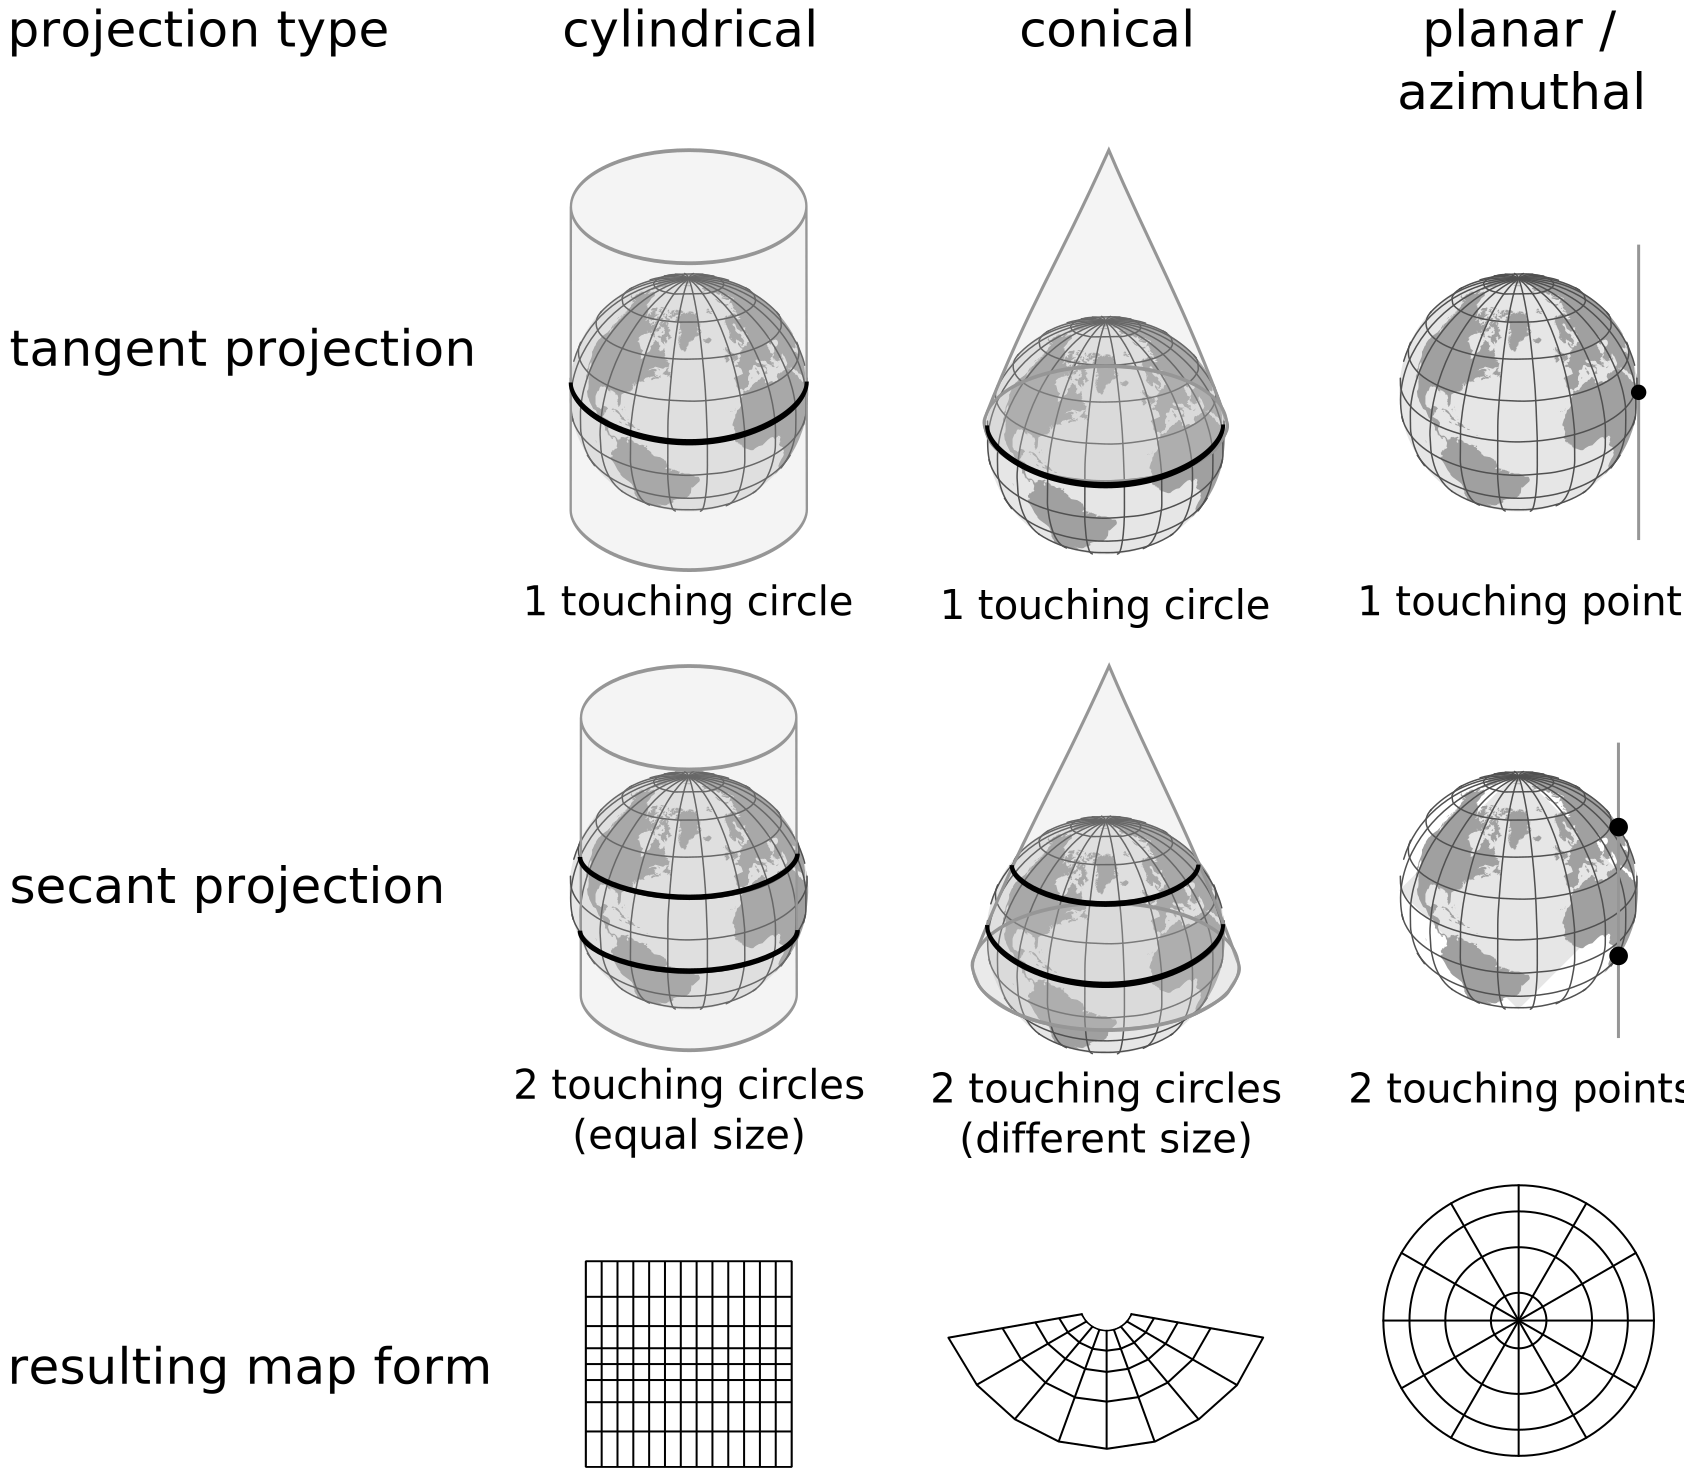
\includegraphics[width=0.73\textwidth]{graphics/basics/projections}
  \caption{Three different developable surfaces for map projections \protect\footnotemark}
  \label{fig:projections}
\end{figure}

\footnotetext{
  based on: \textit{Coordinate Reference Systems},
  QGis Documentation,
  URL: \url{http://docs.qgis.org/2.0/en/docs/gentle_gis_introduction/coordinate_reference_systems.html},
  last access: 27.10.2015
}

In praxis, also pure mathematical map projections are used, e.g. pseudocylindrical, sinusoidal or Mollweise projections. They are much more complex and have the goal to reduce the overall distortion
\cite[p.99]{bolstad2008gis}.

% subsection projection_families (end)


\paragraph{Distortion characteristics} % (fold)
\label{par:distortion_characteristics}

To flatten a spherical surface onto a flat surface, transformations such as stretching, tearing or shearing have to be performed. % affine? non-affine?
A map projection is only accurate at the \emph{standard lines}, i.e. the point(s) or line(s) where the developable surface touches or intersects the ellipsoid. In all other parts the map will in some ways be deformed. That causes distortion in at least one of the following properties of a map: shape (angle), size (area),  direction or distance of features on the map. There is no perfect map projection. Each projection can preserve maximum two of these properties at a cost of distorting the others. The cartographer has to make a compromise and choose a set of characteristics that are important while accepting a distortion in the other properties.

\emph{Tissot's indicatrices} visualize the distortion patterns in the form of ellipses on the map. Their size, shape and orientation are caused by the map projection and show the distortion at this point of the map. Using indicatrices the advantages and disadvantages of each map projection can be shown.

There are two mutual exclusive characteristics: \emph{equivalent} and \emph{conformal}. Equivalent projections preserve the sizes and areas of features on the map, whereas conformal projections preserves angles and the shapes of objects. Every map projection that is area-preserving distorts shapes at the same time, and vice versa
\cite{mapProjectionGeokov}.

\begin{figure}[ht]
  \centering
  \begin{subfigure}{0.59\textwidth}
    \centering
    \includegraphics[width=0.9\linewidth]{graphics/basics/projection_distortion_lambert.png}
    \caption{Lambert cylindrical projection \protect\footnotemark}
  \end{subfigure}
  \begin{subfigure}{0.39\textwidth}
    \centering
    \includegraphics[width=0.9\linewidth]{graphics/basics/projection_distortion_mercator.png}
    \caption{Mercator cylindrical projection \protect\footnotemark}
  \end{subfigure}
  \caption{Comparison of equivalent and conformal map projections}
  \label{fig:lambert_vs_mercator}
\end{figure}

% reset footnotecounter by 1 (for left subfigure caption)
\addtocounter{footnote}{-1}
\footnotetext{
  \textit{Tissot indicatrix world map Lambert cyl equal-area proj},
  Eric Gaba / Sting (Wikimedia), June 2008
  URL: \url{https://commons.wikimedia.org/wiki/File:Tissot_indicatrix_world_map_Lambert_cyl_equal-area_proj.svg},
  last access: 28.10.2015
}

% set footnotecounter to next footnote (for right subfigure caption)
\addtocounter{footnote}{1} % count to next footnote
\footnotetext{
  \textit{Tissot indicatrix world map Mercator proj},
  Eric Gaba / Sting (Wikimedia), September 2008
  URL: \url{https://commons.wikimedia.org/wiki/File:Tissot_indicatrix_world_map_Mercator_proj.svg},
  last access: 28.10.2015
}

The \emph{Mercator projection} (figure \ref{fig:lambert_vs_mercator}b) is an angle-preserving map. It was used for nautical navigation because of a very helpful property: constant compass bearing. A straight line on a Mercator map crosses all meridians in the same angle, a so called \emph{loxodrome}. A navigator only has to follow this line and never needs to reset the compass, because it will always point in the same direction. This is not the shortest way from A to B, but the easiest to navigate. The disadvantage of Mercator maps are the large area distortions towards the poles, which can be seen at the sizes of the ellipses. The best example visualizing the problem is Greenland: On the map it seems almost as large as Africa, whereas in reality Africa is 14 times larger than Greenland.
\cite{mapProjectionGeokov}

This scale becomes obvious in the area-preserving \emph{Lambert projection} (figure \ref{fig:lambert_vs_mercator}a). Tissot's indicatrices all have the same size, but their shapes get distorted towards the poles. This map shows the real size of Africa, but largely distorts the shape of Europe. However, for thematic mapping and teaching purposes equivalent projections are well-suited, because they accurately show the areas of the countries.
\cite{mapProjectionGeokov}

The result of an \emph{equidistant} projection is a map that in relation to the scale accurately shows the distances between certain points on the map.

\vspace{0.5em} % unfortunately necessary to prevent awkward linebreak in footnotes
\begin{figure}[ht]
  \centering
  \begin{subfigure}{0.62\textwidth}
    \centering
    \includegraphics[width=0.9\linewidth]{graphics/basics/projection_distortion_equirectangular.png}
    \caption{Equirectangular equidistant cylindrical projection \protect\footnotemark}
  \end{subfigure}
  \begin{subfigure}{0.37\textwidth}
    \centering
    \includegraphics[width=0.9\linewidth]{graphics/basics/un_logo}
    \caption{Logo of the United Nations \protect\footnotemark}
  \end{subfigure}
  \caption{Two examples of equidistant map projections}
  \label{fig:equidistant_projections}
\end{figure}

% reset footnotecounter by 1 (for left subfigure caption)
\addtocounter{footnote}{-1}
\footnotetext{
  \textit{Tissot indicatrix world map equirectangular proj},
  Eric Gaba / Sting (Wikimedia), June 2008
  URL: \url{https://commons.wikimedia.org/wiki/File:Tissot_indicatrix_world_map_equirectangular_proj.svg},
  last access: 28.10.2015
}

% set footnotecounter to next footnote (for right subfigure caption)
\addtocounter{footnote}{1} % count to next footnote
\footnotetext{
  \textit{Logo of the United Nations},
  Shizhao (Wikimedia), 13.06.2007
  URL: \url{https://commons.wikimedia.org/wiki/File:Logo_of_the_United_Nations_(B\%26W).svg},
  last access: 28.10.2015,
  Comment: This work is excerpted from an official document of the United Nations prior to 17. September 1987.
}

% pidgeon
% irc.freenode.net#slab

Figure \ref{fig:equidistant_projections}b shows a prominent example: The Unites Nations chose a map for their logo from which all points on the map have the correct distance to the North Pole. The equirectangular projection in Figure \ref{fig:equidistant_projections}a has a slightly different property: any meridian is true to scale and therefore all distances along the meridians are accurate. However, the ellipses on the map are distorted in both shape and size, so the map is neither conformal nor equivalent. Air navigation charts or seismology make use of the equidistant property e.g. to show distances from major cities to the epicenter of an earthquake.
\cite{mapProjectionGeokov}

\emph{Zenithal} or \emph{azimuthal} projections preserve directions from the center point to all other points on the map (see figure \ref{fig:zenithal_projection}). It is only possible in the family of planar projections and can be combined with a conformal, equivalent and equidistant property. These maps are used whenever directional relationships are important, for example in navigational charts.

\begin{figure}[ht]
  \centering
  \includegraphics[width=0.3\textwidth]{graphics/basics/projection_distortion_azimuthal.png}
  \caption{Lambert azimuthal (zenithal) equivalent projection \protect\footnotemark}
  \label{fig:zenithal_projection}
\end{figure}

\footnotetext{
  \textit{Lambert azimuthal equal-area projection SW},
  Strebe (Wikimedia), 15. August 2011
  URL: \url{https://commons.wikimedia.org/wiki/File:Lambert_azimuthal_equal-area_projection_SW.jpg},
  last access: 28.10.2015
}

If no characteristic is explicitly important but the overall distortion shall be minimized, a \emph{compromise projection} can be used. They do not preserve any property, but are a trade-off in the distortion of all other properties. The Robinson projection in figure \ref{fig:robinson_projection} is a well-known example. All Tissot's indicatrices not on the Equator are distorted in size, shape and direction, but compared to the Mercator or Lambert projection, the magnitude of distortion is lower.

\begin{figure}[ht]
  \centering
  \includegraphics[width=0.65\textwidth]{graphics/basics/projection_distortion_robinson.png}
  \caption{Robinson projection \protect\footnotemark}
  \label{fig:robinson_projection}
\end{figure}

\footnotetext{
  \textit{Tissot indicatrix world map Robinson},
  Eric Gaba / Sting (Wikimedia), June 2008
  URL: \url{https://commons.wikimedia.org/wiki/File:Tissot_indicatrix_world_map_Robinson_proj.svg},
  last access: 28.10.2015
}

% paragraph map_projections (end)

% subsubsection maps (end)

% ------------------------------------------------------------------------------
\subsubsection{Timelines} % (fold)
\label{ssub:timelines}

% subsubsection timelines (end)

% subsection presentation (end)

% section system_components (end)

% ==============================================================================
\section{Application} % (fold)
\label{sec:application}

In summary,  The research focuses on changes over time triggered by historical events happening in an historical context. There are currently no historical information systems that scientists of this field use for their research, it is rather based on primary and secondary sources, e.h. historical documents, speeches or photography.

\emph{Historical} or \emph{temporal geographic information systems} (HGIS) combine elements of history and geography into one information system to be able to answer research questions for both historians and geographers: ``situating history in its geographical context and using geographic information to illuminate the past.''
\cite[p. 3]{knowles2008placing}
This manifests the interdisciplinary nature of HGIS and making it also an interesting technology in the context of \emph{digital humanities}, the intersection between humanities and computing. The main distinction to classical GIS is the integration of the component of time, making the system four-dimensional. HGIS collect, manage, analyze and present spatio-temporal information and models changes over time and space
\cite[p. xii]{knowles2002past}

there is ``not any operational temporal GIS''
\cite[p. 5]{raza12}

  \emph{lifelines}
    showing tracks, routes and meetings or people -> linear, time steps
    historic example: Napoleons Moscow Campaign
    \includegraphics[width=0.8\textwidth]{graphics/basics/napoleon_march_moscow.png}
    \footnote{
      \textit{Minard.png}
      Charles Minard, 1869,
      URL: \url{https://commons.wikimedia.org/wiki/File:Minard.png},
      last access: 03.11.2015,
      Charles Minard's 1869 chart showing the number of men in Napoleon’s 1812 Russian campaign army, their movements, as well as the temperature they encountered on the return path. Lithograph, 62 x 30 cm
    }
    \cite[pp. 188-191]{knowles2008placing}

  reason about historical events
    combine spatial and temporal and attributional information -> overlays
    e.g. Battlefield stories (what was the cause for the victory of party A?)



HGIS projects
  usage: mostly quantitative research
  -> logical characteristics of information system)

  large collection of research projects
  \cite{knowles2008placing}
  \cite{gregory2014toward}

  ``The Barrington Atlas of the Greek and Roman World''
    gazetteer: name of historic place -> map by map
    \cite{talbert2000barrington}
    \footnote{
      \textit{Ancient World Mapping Center},
      The University of North Carolina,
      URL: \url{http://awmc.unc.edu/},
      last access: 03.11.2015
    }
  solution
    think about how to represent historical knowledge in geographic context
    degree of certainty -> ironically: that has to be exact as well in a database table
    => reason: careful conclusions from historical maps
  problem: tedious manual work
    ~20 hour per map already digitized
    \cite[pp. 145]{knowles2002past}

  show change over time (historical development)
  state-based approach (photography: validity period of geometries)

  ``Great Britain Historical GIS Project'' (GBHGIS)
    \footnote{
      \textit{Great Britain Historical Geographical Information System (GBHGIS)},
      Ian Gregory \& Humphrey R. Southall, University of Portsmouth, since 1994,
      URL: \url{http://www.port.ac.uk/research/gbhgis/},
      last access: 02.11.2015
    }
    idea:
      combine statistical data with territorial units
      => new analytical opportunities
      e.g. analyze net migration in the districts in UK
      -> snapshot model
    problem:
      ``To map and spatially analyze data correctly, quantities must be linked to an accurate representation of the units for which they were collected.''
      administrative units / districts fundamentally changed three times and slightly changed hundreds of times over the last 200 years
      statistical data is gathered per unit
      hardly any info about historical boundaries of districts
      (some by British Ordnance Survey, but not covering everything)
      => results would be disproportional
    \cite[pp. 117-129]{knowles2002past}
    solution: aerial interpolation
      geostatistical interpolation
      discrete data proportional to source polygon (old geometry) -> reaggregate to target polygons (new geometry)
      => prediction
      \cite{aerialInterpolation}

    UK ordnance survey
      * automatic change detection
      \url{https://www.ordnancesurvey.co.uk/education-research/research/automatic-change-detection.html}

  ``National Historical Geographic Information System'' (NHGIS)
    \footnote{
      \textit{Welcome to NHGIS},
      Minnesota Population Center, University of Minnesota,
      since 2007,
      URL: \url{http://www.port.ac.uk/research/gbhgis/},
      last access: 02.11.2015
    }
    idea:
      provide digital boundaries for each census year
      -> estimation of population of any year
    concept:
      composite map: each face represents an area that never changed
      -> composition to regions per year based on compositing information
      dealing with problem of varying administrative borders through aerial interpolation
    interface:
      very scientific a lot of options
      need tutorial to go through the selection
      need to register before downloading something
      get a link to download a file
      have to decompress it
      then load it into your preferred GIS
      -> incredibly frustrating !!!


This application does maps and timelines:

https://www.palantir.com/palantir-gotham/applications/

MAP
The Map application delivers geospatial analytic capabilities. It combines the visualization of geo-located objects on a map with histogram, timeline and time wheel visualizations. A heatmap visualization illuminates the density of interesting objects on the map.

The imagery on the Map is fully pluggable, allowing users to switch between different sources of imagery, integrate private imagery, and create composite imagery sets that combine two or more sources of imagery.

KML and Shapefiles can be imported as independent map layers, and shapes contained in these layers can be used to select and filter objects that lie in a similar region (like a county, census plot, or state). Layers can be colored and labeled according to calculations performed on the data they contain.


Here is a group using the tool to do historical maps: http://envisioninghistory.org/


And here is a program I’m using for my dissertation. I don’t know if it does timelines and maps, but I think it might.

http://www.tableau.com/

Here are some examples of what I’m doing with it:
% https://public.tableau.com/profile/ammon.shepherd#!/

And my dissertation website just for fun: http://nazitunnels.org

The major problem that lays in the nature of the qualitative historical research is that all historic sources are subjective and biased, their content may be fuzzy and they are definitely incomplete. So the knowledge that can be extracted from a source bears the integral problem of \emph{uncertainty}. On the other hand there are information systems with a logical architecture, with the goal to be as precise and accurate as possible. Analysis is based on mathematical functions -- in its entire nature an information system is quantitative. This contrast is the main problem why HGIS is not widely accepted yet
\cite[p. 2]{knowles2008placing}.

Another problem for historians is that they do not necessarily need a tool to better visualize existing knowledge (e.g. historical maps), but to generate new knowledge by analyzing spatio-temporal coherences or distributions in historical data. Spatio-temporal reasoning is still an open field and not easily possible with existing HGIS
\cite[p. 268]{knowles2008placing}, \cite[p. xii]{gregory2014toward}.

Some interesting research questions that could be answered using HGIS could be:

\begin{itemize}
  \item Did the European Union help to bring peace on the European continent or the other way around? (political)
  \item Is there a coherence between life expectancy and fertility rate on earth? (social)
  \item Does global warming speed up the melting of the glaciers? (physical)
  \item What was the contribution of Bismarck's foreign policy to a longer period of peace in Europe from 1871 to 1914? (historical)
\end{itemize}

Or on a more abstract level: Where and When has something changed and why did it change?


space-time premise by Gaddis 2002
  time and space equal importance
  event     what significantly has happend and by whom? (singularity!)
  process   how something has happened? (event+activity => trigger of process)
  change    driven by process
  spatiotemporal data defines all above three
  % \cite Gaddis 2002


% ------------------------------------------------------------------------------
\subsection{Digital Humanities} % (fold)
\label{sub:digital_humanities}

% subsection digital_humanities (end)

% ------------------------------------------------------------------------------
\subsection{HistoGlobe} % (fold)
\label{sub:histoglobe}

% subsection histoglobe (end)

% section application (end)


\vspace{2em}

transition to concept chapter